%By Kevin Cheung
%The book is licensed under the
%\href{http://creativecommons.org/licenses/by-sa/4.0/}{Creative Commons
%Attribution-ShareAlike 4.0 International License}.
%
%This file has been modified by Robert Hildebrand 2020.  
%CC BY SA 4.0 licence still applies.

\section{Graphical example}\label{graphic}

To motivate the subject of linear programming (LP), we begin with a
planning problem that can be solved graphically.

Say you are a vendor of lemonade and lemon juice. Each unit of lemonade
requires 1 lemon and 2 litres of water. Each unit of lemon juice
requires 3 lemons and 1 litre of water. Each unit of lemonade gives a
profit of three dollars. Each unit of lemon juice gives a profit of two
dollars. You have 6 lemons and 4 litres of water available. How many
units of lemonade and lemon juice should you make to maximize profit?

If we let \(x\) denote the number of units of lemonade to be made and
let \(y\) denote the number of units of lemon juice to be made, then the
profit is given by \(3x + 2y\) dollars. We call \(3x + 2y\) the
objective function. Note that there are a number of constraints that
\(x\) and \(y\) must satisfied. First of all, \(x\) and \(y\) should be
nonnegative. The number of lemons needed to make \(x\) units of lemonade
and \(y\) units of lemon juice is \(x+3y\) and cannot exceed 6. The
number of litres of water needed to make \(x\) units of lemonade and
\(y\) units of lemon juice is \(2x+y\) and cannot exceed 4. Hence, to
determine the maximum profit, we need to maximize \(3x + 2y\) subject to
\(x\) and \(y\) satisfying the constraints \(x + 3y \leq 6\),
\(2x + y \leq 4\), \(x \geq 0\), and \(y \geq 0.\)

A more compact way to write the problem is as follows:
\[\begin{array}{rrcrll}
\mbox{maximize } & 3x & + & 2y & \\
\mbox{subject to} 
& x & + & 3y & \leq & 6 \\
& 2x & +&  y & \leq & 4 \\
& x &  & & \geq & 0 \\
& & & y & \geq & 0. \\
\end{array}\]

We can solve this maximizationproblem graphically as follows. We first
sketch the set of \(\begin{bmatrix} x\\ y\end{bmatrix}\) satisfying the
constraints, called the feasible region, on the \((x,y)\)-plane. We then
take the objective function \(3x+2y\) and turn it into an equation of a
line \(3x+2y = z\) where \(z\) is a parameter. Note that as the value of
\(z\) increases, the line defined by the equation \(3x+2y=z\) moves in
the direction of the normal vector
\(\begin{bmatrix} 3 \\ 2\end{bmatrix}\). We call this direction the
direction of improvement. Determining the maximum value of the objective
function, called the optimal value, subject to the contraints amounts to
finding the maximum value of \(z\) so that the line defined by the
equation \(3x+2y=z\) still intersects the feasible region.

\begin{center}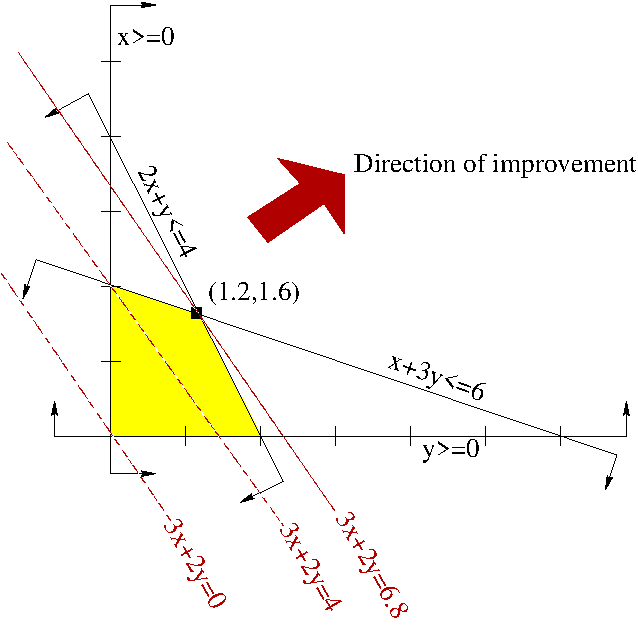
\includegraphics[width=0.8\linewidth]{images/lemon} \end{center}

In the figure above, the lines with \(z\) at 0, 4 and 6.8 have been
drawn. From the picture, we can see that if \(z\) is greater than 6.8,
the line defined by \(3x+2y = z\) will not intersect the feasible
region. Hence, the profit cannot exceed 6.8 dollars.

As the line \(3x+2y = 6.8\) does intersect the feasible region, \(6.8\)
is the maximum value for the objective function. Note that there is only
one point in the feasible region that intersects the line \(3x+2y=6.8\),
namely
\(\begin{bmatrix} x \\ y\end{bmatrix} = \begin{bmatrix} 1.2 \\ 1.6\end{bmatrix}.\)
In other words, to maximize profit, we want to make 1.2 units of
lemonade and 1.6 units of lemon juice.

The above solution method can hardly be regarded as rigorous because we
relied on a picture to conclude that \(3x + 2y \leq 6.8\) for all
\(\begin{bmatrix} x\\y\end{bmatrix}\) satisfying the constraints. But we
can actually show this \emph{algebraically}.

Note that multiplying both sides of the constraint \(x + 3y \leq 6\)
gives \(0.2x + 0.6 y \leq 1.2\), and multiplying both sides of the
constraint \(2x + y \leq 4\) gives \(2.8x + 1.4 y \leq 5.6\). Hence, any
\(\begin{bmatrix} x\\y\end{bmatrix}\) that satisfies both \(x+3y\leq 6\)
and \(2x+y \leq 4\) must also satisfy
\((0.2x+0.6y) + (2.8x+1.4y) \leq 1.2 + 5.6\), which simplifies to
\(3x + 2y \leq 6.8\) as desired! (Here, we used the fact that if
\(a \leq b\) and \(c \leq d\), then \(a+c \leq b+d\).)

Now, one might ask if it is always possible to find an algebraic proof
like the one above for similar problems. If the answer is yes, how does
one find such a proof? We will see answers to this question later on.

Before we end this segment, let us consider the following problem:
\[\begin{array}{rrcrll}
\mbox{minimize } & -2x & + & y & \\
\mbox{subject to} & -x & + & y & \leq & 3 \\
& x & - &  2y & \leq & 2 \\
& x &  & & \geq & 0 \\
& & & y & \geq & 0. \\
\end{array}\]

Note that for any \(t \geq 0\),
\(\begin{bmatrix} x \\ y\end{bmatrix} = \begin{bmatrix} t \\ t\end{bmatrix}\)
satisfies all the constraints. The value of the objective function at
\(\begin{bmatrix} x \\ y\end{bmatrix} = \begin{bmatrix} t \\ t\end{bmatrix}\)
is \(-t\). As \(t \rightarrow \infty\), the value of the objective
function tends to \(-\infty\). Therefore, there is no minimum value for
the objective function. The problem is said to be unbounded. Later on,
we will see how to detect unboundedness algorithmically.

As an exercise, check that unboundedness can also be established by
using
\(\begin{bmatrix} x \\ y\end{bmatrix} = \begin{bmatrix} 2t+2 \\ t\end{bmatrix}\)
for \(t \geq 0\).

\subsection*{Exercises}\label{exercises}
\addcontentsline{toc}{section}{Exercises}

\begin{enumerate}
\def\labelenumi{\arabic{enumi}.}
\item
  Sketch all \(\begin{bmatrix} x \\ y \end{bmatrix}\) satisfying

  \begin{equation*}
  x - 2y \leq 2
  \end{equation*}

  on the \((x,y)\)-plane.
\item
  Determine the optimal value of \[
  \begin{array}{rl}
  \text{Minimize} & x + y \\
  \text{Subject to} &  2x + y \geq 4 \\
  & x + 3y \geq 1.
  \end{array}
  \]
\item
  Show that the problem \[
  \begin{array}{rl}
  \text{Minimize} & -x + y \\
  \text{Subject to} &  2x - y \geq 0 \\
  & x + 3y \geq 3
  \end{array}
  \] is unbounded.
\item
  Suppose that you are shopping for dietary supplements to satisfy your
  required daily intake of 0.40mg of nutrient \(M\) and 0.30mg of
  nutrient \(N\). There are three popular products on the market. The
  costs and the amounts of the two nutrients are given in the following
  table:

  \begin{longtable}[]{@{}lccc@{}}
  \toprule
  & Product 1 & Product 2 & Product 3\tabularnewline
  \midrule
  \endhead
  Cost & \$27 & \$31 & \$24\tabularnewline
  Daily amount of \(M\) & 0.16 mg & 0.21 mg & 0.11 mg\tabularnewline
  Daily amount of \(N\) & 0.19 mg & 0.13 mg & 0.15 mg\tabularnewline
  \bottomrule
  \end{longtable}

  You want to determine how much of each product you should buy so that
  the daily intake requirements of the two nutrients are satisfied at
  minimum cost. Formulate your problem as a linear programming problem,
  assuming that you can buy a fractional number of each product.
\end{enumerate}

\subsection*{Solutions}\label{solutions}
\addcontentsline{toc}{subsection}{Solutions}

\begin{enumerate}
\def\labelenumi{\arabic{enumi}.}
\item
  The points \((x,y)\) satisfying \(x-2y \leq 2\) are precisely those
  above the line passing through \((2,0)\) and \((0,-1)\).
\item
  We want to determine the minimum value \(z\) so that \(x+y=z\) defines
  a line that has a nonempty intersection with the feasible region.
  However, we can avoid referring to a sketch by setting \(x=z-y\) and
  substituting for \(x\) in the inequalities to obtain:

  \begin{eqnarray*}
   2(z-y) + y \geq 4 \\
   (z-y) + 3y \geq 1,
  \end{eqnarray*}

  or equivalently,

  \begin{eqnarray*}
   z \geq 2+\frac{1}{2}y \\
   z \geq 1-2y,
  \end{eqnarray*}

  Thus, the minimum value for \(z\) is
  \(\min \{ 2+\frac{1}{2}y, 1-2y\}\), which occurs at
  \(y = -\frac{2}{5}\). Hence, the optimal value is \(\frac{9}{5}\).

  We can verify our work by doing the following. If our calculations
  above are correct, then an optimal solution is given by
  \(x = \frac{11}{5}\), \(y = -\frac{2}{5}\) since \(x = z - y\). It is
  easy to check that this satisfies both inequalities and therefore is a
  feasible solution.

  Now, taking \(\frac{2}{5}\) times the first inequality and
  \(\frac{1}{5}\) times the second inequality, we can infer the
  inequality \(x+y \geq \frac{9}{5}\). The left-hand side of this
  inequality is precisely the objective function. Hence, no feasible
  solution can have objective function value less than \(\frac{9}{5}\).
  But \(x = \frac{11}{5}\), \(y = -\frac{2}{5}\) is a feasible solution
  with objective function value equal to \(\frac{9}{5}\). As a result,
  it must be an optimal solution.

  \textbf{Remark.} We have not yet discussed how to obtain the
  multipliers \(\frac{2}{5}\) and \(\frac{1}{5}\) for inferring the
  inequality \(x+y \geq \frac{9}{5}\). This is an issue that will be
  taken up later. In the meantime, think about how one could have
  obtained these multipliers for this particular exercise.
\item
  We could glean some insight by first making a sketch on the
  \((x,y)\)-plane.

  The line defined by \(-x + y = z\) has \(x\)-intercept \(-z\). Note
  that for \(z \leq -3\),
  \(\begin{bmatrix} x\\y \end{bmatrix} = \begin{bmatrix} -z\\ 0\end{bmatrix}\)
  satisfies both inequalities and the value of the objective function at
  \(\begin{bmatrix} x\\y \end{bmatrix} = \begin{bmatrix} -z\\ 0\end{bmatrix}\)
  is \(z\). Hence, there is no lower bound on the value of objective
  function.
\item
  Let \(x_i\) denote the amount of Product \(i\) to buy for
  \(i = 1,2,3\). Then, the problem can be formulated as
  \[\begin{array}{rrcrcrll}
  \mbox{minimize } & 27 x_1 & + & 31 x_2 & + & 24 x_3 \\
  \mbox{subject to} 
  & 0.16 x_1 & + & 0.21 x_2 & + & 0.11 x_3 & \geq & 0.30 \\
  & 0.19 x_1 & + & 0.13 x_2 & + & 0.15 x_3 & \geq & 0.40 \\
  & x_1 & , & x_2 & , & x_3 & \geq & 0. \\
  \end{array}\]

  \textbf{Remark.} If one cannot buy fractional amounts of the products,
  the problem can be formulated as \[\begin{array}{rrcrcrll}
  \mbox{minimize } & 27 x_1 & + & 31 x_2 & + & 24 x_3 \\
  \mbox{subject to} 
  & 0.16 x_1 & + & 0.21 x_2 & + & 0.11 x_3 & \geq & 0.30 \\
  & 0.19 x_1 & + & 0.13 x_2 & + & 0.15 x_3 & \geq & 0.40 \\
  & x_1 & , & x_2 & , & x_3 & \geq & 0. \\
  & x_1 & , & x_2 & , & x_3 & \in & \mathbb{Z}. \\
  \end{array}\]
\end{enumerate}